\documentclass[11pt,a4paper]{report}

\usepackage{lmodern}
\usepackage{amsmath, amsfonts}

\usepackage{tikz}

\begin{document}
\title{A Speech Command System on PR2}
\author{Weipeng He, Natalia Orlova}
\maketitle

\begin{abstract}
  In this report we would like to present the theories and implementations of our speech recognition system on PR2. 
\end{abstract}

\tableofcontents

\listoffigures

\chapter{Introduction}

\chapter{Speech Processing Basics}
\section{Short Time Fourier Transform}

\section{Implementation of Audio I/O System}
Although there are plenty of literatures about the theories of audio processing, there rarely are detailed documents on how the systems are implemented. To close the gap between theories and implementation, in this section, we would like to address the basic concepts of audio programming as well as details of the implementation of basic audio input and output in our system.

Theories of audio processing are always seemed to be neat and appealing. However, when it comes to writing a program to realize an algorithm, much more ``dirty'' works will be involved. These extra works are largely due to handling of hardware status and numerical computing, which are sometimes neglected in theories.

In this section, we will first introduce the basic concepts of digital audio signal processing. Afterward, we will show how to implement a minimal audio recording program using the Advanced Linux Sound Architecture (ALSA).

\subsection{Sampling and PCM}
To process an audio signal, first of all, we need to know how the signal is represented. Ideally, the audio signal is just amplitudes over time (time-domain signal), namely $ x(t) \in \mathbb{R},~ t \in \mathbb{R} $. However, practically, we need to represent the signal discretely. Thus, discretization on both time and amplitude (\textit{sampling} and \textit{quantization}, respectively) should be applied. As the result, the signal is represented using a sequence of quantized values $x_n$.

For sampling, we take the values of the continuous signal using a \textit{sampler} at $T_s$ time intervals: \[ x_s[n] = x(n T_c) \in \mathbb{R},~ n \in \mathbb{Z} \] Here, $T_s$ is called the \textit{sampling period}, and $ f_s = \frac{1}{T_c} $ is called the \textit{sampling frequency}.

After sampling, the \textit{A/D converter} converts the real values to a limited set of values, which can be represented by binary data. In digital audio, \textit{Pulse-code modulation} (PCM) is the most common method for this quantization process. 

PCM has several quantization methods, which includes Linear PCM, A-law algorithm or $\mu$-law algorithm. Although different algorithms exist, PCM sometimes refer to Linear PCM by default as it is the most popular. Linear PCM quantize each sample using linearly uniform levels. In other words, all adjacent levels have the same difference in sound amplitude. The number of levels depends on the bit depth of each code.

Within each quantization method, different encoding method, e.g. \textit{format}, can be chosen. These formats are named according to the bit depth, endianness, float/integer and signed/unsigned that they use. For example, a format can be 32 bits signed integer with little endian. Some applications and libraries, such as aplay, ALSA, gstreamer, use a short name for each format. As for the example format, the name is ``\texttt{S32\_LE}''. The structure of the format name is shown in Figure \ref{fig:pcmname}. Other common formats includes \texttt{S8}, \texttt{U8}, \texttt{S16\_LE}, \texttt{F32\_LE}, \texttt{F64\_LE}, etc.

\begin{figure}[htpb]
\begin{center}
  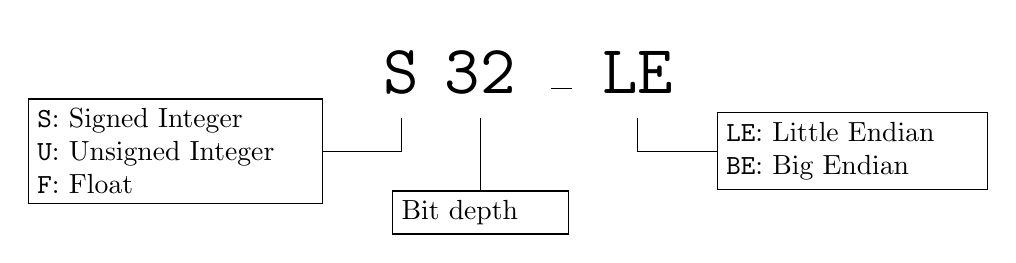
\begin{tikzpicture}
    {\Huge\texttt{
      \node(s) at (0,0) {S};
      \node(b) at (1,0) {32};
      \node at (2,-0.2) {\_};
      \node(e) at (3,0) {LE};
    }}
    \draw (-1,-1) node[left,text width=3.5cm,draw,rectangle]
       {\texttt{S}: Signed Integer\\\texttt{U}: Unsigned Integer\\\texttt{F}: Float} -| (s.south);
    \draw (1,-1.5) node[below,text width=2cm,draw,rectangle]
       {Bit depth} -- (b.south);
    \draw (4,-1) node[right,text width=3.2cm,draw,rectangle]
       {\texttt{LE}: Little Endian\\\texttt{BE}: Big Endian} -| (e.south);
  \end{tikzpicture}
\end{center}
\caption[Name structure of PCM format.]{Name structure of PCM format. The first letter represents the data type. Then follows a number, which is the bit depth of each sample. If the bit depth is larger than 8 (1 byte), then there is a tag, which states the endianness, at the end.}
  \label{fig:pcmname}
\end{figure}

Now, we can represent a single channeled audio recording using a sequence of PCM binary data. Furthermore, for multi-channeled audio recording, it it just simple interleave the data of each channel. A set of samples at one time from all channels is called a \textit{frame}. For example, suppose we have a 2-channeled data using \texttt{S16\_LE} format. Then the first 2 bytes are the first sample of channel 1, and the second 2 bytes are the first sample of channel 2. Thus, bytes number 1 to 4, are the first frame. And, the second samples of both channels are at the number 5 to 8 bytes, which consist the second frame. And so on.

To summarize, an audio recording can be represented by binary data using PCM. To sufficiently understand how the audio are encoded, we need to know the following parameters: sampling rate, number of channels and PCM format.

\subsection{Advanced Linux Sound Architecture}
Advanced Linux Sound Architecture (ALSA) is the software framework that provides API for sound device drivers as part of the linux kernel. The API includes configuration of the hardware and write/read audio data.

Besides the aforementioned parameters for audio representation (sampling rate, number of channels and PCM format), some other parameters regarding the hardware buffer are also need to be configured. These parameters are period size and buffer size. As it could be very costly for CPU to fetch the data one sample at a time, normally there is a hardware interrupt every interval. The number of frames that is in this interval is called the \textit{period size}. These data are stored in a ring buffer, and its size if called \textit{buffer size}. Usually the buffer size is twice as the period size. However, it can sometimes be up to 8 times of that.

% \subsection{Implementation using ALSA}

\chapter{Sound Source Separation}


\chapter{Noise Reduction Techniques}

\chapter{Conclusion}


\bibliographystyle{plain}
\bibliography{project}
 
\end{document}
